\chapter{Corrélations d’Ising, champ moyen et aimantation spontanée}

\lectureoverview{Une chaîne d’Ising unidimensionnelle se résout exactement en remplaçant les spins des sites par des variables de liaison. Ce changement de variables transforme la fonction de partition en un produit et montre qu’à toute température finie, les corrélations décroissent exponentiellement. Les réseaux de dimension supérieure se comportent différemment, car chaque spin reçoit des informations de nombreux voisins. En traitant leur influence combinée comme un champ moyen, on obtient une équation d’autocohérence, une température critique de champ moyen et une description précise de la façon dont un champ extérieur arbitrairement faible sélectionne une phase aimantée.}

\section{Ce qu’Ising a réellement établi}

Le point historique doit être énoncé avec précision. Ernst Ising a résolu le modèle unidimensionnel proposé par Wilhelm Lenz et a correctement conclu à l’absence de transition de phase à température finie. C’est en extrapolant que l’on a eu tort de déduire que la même conclusion s’appliquait à toutes les dimensions. Ce n’est pas le cas. Le modèle bidimensionnel présente déjà une phase ordonnée à basse température.

Une solution exacte en dimension supérieure serait trop ambitieuse pour le moment. Une approximation physiquement intuitive suffira à mettre en évidence la transition lorsque chaque spin a de nombreux voisins. Avant de faire cette approximation, il convient toutefois de résoudre exactement la chaîne unidimensionnelle. Le contraste entre la solution exacte en une dimension et l’approximation en grande dimension fait ressortir le mécanisme absent en une dimension.

Ici, une transition de phase désigne davantage qu’un renforcement graduel d’une préférence déjà présente. Lorsque la température franchit une valeur critique, l’état d’équilibre acquiert une nouvelle propriété macroscopique : une aimantation non nulle peut subsister même après le retrait du champ extérieur qui a servi à orienter l’échantillon. Le calcul doit donc répondre à deux questions distinctes. Un spin éloigné garde-t-il en mémoire l’orientation d’un spin choisi, et un champ infinitésimal peut-il organiser un échantillon arbitrairement grand ?

\section{Le spin unique comme brique de base réutilisable}

Considérons une variable à deux états
\begin{equation}
\sigma=\pm1,
\end{equation}et choisissons la convention d’énergie
\begin{equation}
E(\sigma)=-J\sigma,
\qquad J>0.
\end{equation}L’état \(\sigma=+1\) est alors celui de plus basse énergie. Le paramètre \(J\) peut représenter le produit d’un moment magnétique par un champ appliqué, mais seul ce produit intervient dans le calcul.

Considérons ce spin comme un petit sous-système en équilibre thermique avec tout le reste. Sa fonction de partition est
\begin{align}
z
&=\sum_{\sigma=\pm1}e^{-\beta E(\sigma)}
 =\sum_{\sigma=\pm1}e^{\beta J\sigma} \\
&=e^{\beta J}+e^{-\beta J}
 =2\cosh(\beta J).
\end{align}

On pourrait obtenir le même résultat en considérant un ensemble de \(N\) spins indépendants. La fonction de partition totale serait simplement \(Z=z^N\), d’où \(\log Z=N\log z\) ; chaque grandeur thermodynamique extensive serait alors égale à \(N\) fois sa valeur pour un spin. Cette approche par sous-système remplace le dénombrement combinatoire plus long du nombre de spins orientés vers le haut et vers le bas, mais contient la même information.
L’énergie moyenne découle de la dérivée logarithmique :
\begin{align}
\expect{E}
&=-\frac{\partial}{\partial\beta}\log z \\
&=-J\frac{\sinh(\beta J)}{\cosh(\beta J)}
 =-J\tanh(\beta J).
\end{align}
Puisque \(E=-J\sigma\),
\begin{equation}
\expect{\sigma}=\tanh(\beta J).
\end{equation}

\begin{figure}[ht]\centering
\includegraphics[width=0.80\textwidth]{lecture_09_figure_02.png}\caption{L’énergie et l’aimantation d’un spin, sous la forme d’une tangente hyperbolique.}\lectureframe{00:10:06}\end{figure}

Cette formule unique englobe les deux limites de température. À basse température, \(\beta J\gg1\), et le spin se trouve presque certainement dans l’état de plus basse énergie. À haute température, \(\beta J\ll1\), donc
\begin{equation}
\expect{\sigma}\simeq \beta J\longrightarrow0.
\end{equation}
L’agitation thermique efface le biais énergétique.

\begin{classroomqa}\audiencequestion{L’énergie moyenne doit-elle comporter un signe moins ?}\lecturerresponse{Oui. L’identité thermodynamique est \(\expect{E}=-\partial_\beta\log z\), le résultat est donc \(-J\tanh(\beta J)\). En divisant ensuite par le facteur \(-J\) dans \(E=-J\sigma\), on obtient l’aimantation positive \(\expect{\sigma}=\tanh(\beta J)\). \lecturetimestamp{00:09:15--00:09:44}}\end{classroomqa}

\section{La chaîne unidimensionnelle}

Plaçons \(N\) spins sur une chaîne ouverte et faisons interagir les spins voisins :
\begin{equation}
H=-J\sum_{i=1}^{N-1}\sigma_i\sigma_{i+1},
\qquad \sigma_i=\pm1.
\label{eq:ising-chain}
\end{equation}
Pour \(J>0\), une paire de spins parallèles contribue \(-J\), tandis qu’une paire antiparallèle contribue \(+J\). Les deux états fondamentaux sont donc
\begin{equation}
(+,+,\ldots,+)
\qquad\text{and}\qquad
(-,-,\ldots,-).
\end{equation}

\begin{figure}[ht]\centering
\includegraphics[width=0.80\textwidth]{lecture_09_figure_03.png}\caption{L’hamiltonien de la chaîne ouverte et sa somme de Boltzmann.}\lectureframe{00:19:15}\end{figure}

Remplacer \(J\) par \(-J\) favorise l’alternance des spins. Sur une chaîne ouverte ou une chaîne périodique de longueur paire, la redéfinition
\begin{equation}
\widetilde{\sigma}_i=(-1)^i\sigma_i
\end{equation}
transforme le signe antiferromagnétique en signe ferromagnétique. La distinction est physique, mais l’algèbre de la fonction de partition unidimensionnelle reste la même. Une chaîne périodique de longueur impaire constitue l’exception habituelle, car elle ne peut alterner sans frustration.

\begin{classroomqa}\audiencequestion{Y a-t-il un champ magnétique extérieur dans l’hamiltonien de la chaîne ?}\lecturerresponse{Pas encore. L’équation~\eqref{eq:ising-chain} ne contient que le couplage entre plus proches voisins. Nous ajouterons plus tard un champ extérieur uniforme sous la forme d’un terme distinct, \(-h\sum_i\sigma_i\), précisément pour tester la réponse de l’état ordonné à un biais arbitrairement faible. \lecturetimestamp{00:18:54--00:19:13}}\end{classroomqa}

\subsection{La mémoire comme fonction de corrélation}

Supposons que \(\sigma_i\) soit connu comme étant orienté vers le haut. Cette information influence-t-elle un spin situé à \(r\) liaisons de distance ? Le diagnostic est
\begin{equation}
C(r)=\expect{\sigma_i\sigma_{i+r}}.
\end{equation}
Si \(C(r)\) tend vers une valeur non nulle lorsque \(r\to\infty\), le système conserve une mémoire à longue portée. Si cette fonction tend vers zéro, l’influence du premier spin finit par disparaître.

Le jeu du téléphone donne la bonne intuition. Chaque personne transmet un symbole binaire à la suivante. Si chaque transmission est parfaite, le bit initial subsiste indéfiniment. Si chaque étape comporte une probabilité d’erreur non nulle, les transmissions répétées finissent par faire perdre le message initial. La température nulle correspond à la limite de transmission parfaite de la chaîne d’Ising. Toute température positive autorise des désaccords occasionnels entre voisins.

Pour illustrer cela numériquement, supposons que la fidélité d’une transmission soit \(0.99\). La probabilité de deux transmissions parfaites est \(0.99^2=0.9801\), et chaque étape supplémentaire apporte un facteur \(0.99\). Au bout de cent étapes, les erreurs sont déjà fréquentes ; dix mille étapes suffisent à effacer toute mémoire pratique. La chaîne d’Ising utilise une mesure signée de la fidélité, plutôt que la probabilité d’absence d’erreur, mais l’idée de la perte multiplicative est la même.

L’analogie devient exacte si l’on distingue une probabilité d’une corrélation. Si \(p\) est la probabilité que deux spins voisins soient parallèles, alors
\begin{equation}
\expect{\sigma_i\sigma_{i+1}}
=p-(1-p)=2p-1.
\end{equation}
La quantité qui se multiplie de liaison en liaison est donc la fidélité excédentaire \(2p-1\), et non \(p\) elle-même.

\section{Variables de liaison et fonction de partition exacte}

Le changement de variables décisif consiste à décrire les relations plutôt que les spins individuels :
\begin{equation}
\mu_i=\sigma_i\sigma_{i+1},
\qquad i=1,\ldots,N-1.
\label{eq:bond-variable}
\end{equation}
Chaque variable de liaison vaut \(+1\) si les spins sont parallèles et \(-1\) s’ils sont antiparallèles. Si le premier spin est fixé, les variables de liaison déterminent tous les spins suivants :
\begin{align}
\sigma_2&=\sigma_1\mu_1,\\
\sigma_3&=\sigma_1\mu_1\mu_2,\\
\sigma_{r+1}&=\sigma_1\prod_{k=1}^{r}\mu_k.
\end{align}
Il n’y a pas de redondance. Les données \((\sigma_1,\mu_1,\ldots,\mu_{N-1})\) équivalent à \((\sigma_1,\ldots,\sigma_N)\).

Dans ces variables, l’énergie s’écrit simplement
\begin{equation}
H=-J\sum_{i=1}^{N-1}\mu_i.
\end{equation}
Les variables de spin couplées sur les sites sont devenues des variables de liaison indépendantes. En sommant d’abord sur les deux valeurs de \(\sigma_1\), on obtient
\begin{align}
Z_N
&=2\sum_{\{\mu_i=\pm1\}}
\exp\left(\beta J\sum_{i=1}^{N-1}\mu_i\right)\\
&=2\prod_{i=1}^{N-1}
\left(\sum_{\mu_i=\pm1}e^{\beta J\mu_i}\right)\\
&=2\left[2\cosh(\beta J)\right]^{N-1}.
\label{eq:chain-partition}
\end{align}
Il y a \(N-1\) facteurs, car une chaîne ouverte de \(N\) sites comporte \(N-1\) liaisons.

Le facteur deux initial correspond au choix global du premier spin. Il ne contribue que \(\log2\) à \(\log Z_N\), tandis que les variables de liaison apportent un terme proportionnel à \(N-1\). Ce facteur compte pour le dénombrement exact à taille finie, mais disparaît de la densité d’énergie libre lorsque \(N\to\infty\). C’est pourquoi le tableau pouvait le qualifier de « détail sans importance » sans pour autant le supprimer.

\begin{figure}[ht]\centering
\includegraphics[width=0.82\textwidth]{lecture_09_figure_04.png}\caption{L’hamiltonien sur les sites réécrit comme une somme de variables de liaison indépendantes, et la fonction de partition qui en résulte, sous forme factorisée.}\lectureframe{00:35:35}\end{figure}

\begin{classroomqa}\audiencequestion{Qu’est devenue la somme dans l’exposant lorsque le résultat final a pris la forme d’une puissance ?}\lecturerresponse{Elle est d’abord devenue un produit :
\[
e^{\beta J\sum_i\mu_i}=\prod_i e^{\beta J\mu_i}.
\]
La somme sur toutes les configurations des liaisons se sépare alors en une somme de deux termes pour chaque liaison. Puisque chaque facteur vaut \(2\cosh(\beta J)\), le produit est égal à cette quantité à la puissance \((N-1)\). Écrire explicitement le cas de trois spins et deux liaisons rend la factorisation tout à fait manifeste. \lecturetimestamp{00:33:25--00:35:36}}\end{classroomqa}

Il s’agit d’une simple description duale : les variables couplées des sites sont remplacées par des variables découplées des liaisons. Le terme \emph{dualité} convient, car un même système possède deux descriptions dont les degrés de liberté ont des aspects très différents. Ici, c’est un changement exact de variables pour une chaîne unidimensionnelle ouverte.

Dans le langage des réseaux, les variables initiales se trouvent sur les sommets et les nouvelles sur les arêtes. Le choix global du premier spin est la donnée supplémentaire nécessaire pour reconstruire les sommets à partir des arêtes. Cet échange entre sites et liaisons illustre modestement un principe qui devient beaucoup plus puissant en mécanique statistique en dimension supérieure.

\subsection{Fidélité entre plus proches voisins}

Toutes les liaisons ont la même distribution,
\begin{equation}
\begin{aligned}
\Pr(\mu=+1)&=\frac{e^{\beta J}}{2\cosh(\beta J)},\\
\Pr(\mu=-1)&=\frac{e^{-\beta J}}{2\cosh(\beta J)}.
\end{aligned}
\end{equation}
Par conséquent,
\begin{equation}
\expect{\mu_i}
=\expect{\sigma_i\sigma_{i+1}}
=\tanh(\beta J).
\label{eq:nearest-correlation}
\end{equation}

\begin{figure}[ht]\centering
\includegraphics[width=0.80\textwidth]{lecture_09_figure_05.png}\caption{La corrélation entre plus proches voisins exprimée comme la valeur moyenne de la variable de liaison.}\lectureframe{00:36:52}\end{figure}

La probabilité que deux voisins soient parallèles est donc
\begin{equation}
p_{\rm same}
=\frac{1+\tanh(\beta J)}{2}.
\end{equation}
Elle dépasse un demi pour \(J\) positif, tend vers un à température nulle et vaut un demi à température infinie.

\begin{classroomqa}\audiencequestion{Pourquoi une corrélation positive entre plus proches voisins signifie-t-elle que les spins préfèrent être parallèles plutôt qu’antiparallèles ?}\lecturerresponse{Pour \(J>0\), une liaison parallèle a une énergie \(-J\), tandis qu’une liaison antiparallèle a une énergie \(+J\). La valeur positive de \(\expect{\mu}\) indique que \(\mu=+1\), et donc l’alignement, est plus fréquent. Le fait qu’un matériau réel présente un couplage ferromagnétique ou antiferromagnétique dépend de sa structure électronique microscopique ; la convention de signe adoptée ici décrit un ferromagnétique. \lecturetimestamp{00:43:45--00:44:48}}\end{classroomqa}

\begin{classroomqa}\audiencequestion{Que devient cette corrélation à très haute température ?}\lecturerresponse{Lorsque \(T\to\infty\), \(\beta\to0\) et \(\tanh(\beta J)\to0\). Même les plus proches voisins ne portent alors aucune information les uns sur les autres : chaque spin revient effectivement à un choix aléatoire. \lecturetimestamp{00:46:42--00:47:20}}\end{classroomqa}

\subsection{Corrélation à grande distance}

Pour des spins séparés par \(r\) liaisons,
\begin{align}
\sigma_i\sigma_{i+r}
&=\sigma_i
\left(\prod_{k=i+1}^{i+r-1}\sigma_k^2\right)
\sigma_{i+r}\\
&=(\sigma_i\sigma_{i+1})
(\sigma_{i+1}\sigma_{i+2})\cdots
(\sigma_{i+r-1}\sigma_{i+r})\\
&=\prod_{k=i}^{i+r-1}\mu_k.
\end{align}
Comme les \(\mu_k\) sont indépendantes,
\begin{equation}
C(r)=\expect{\sigma_i\sigma_{i+r}}
=\left[\tanh(\beta J)\right]^r.
\label{eq:exact-correlation}
\end{equation}

\begin{figure}[ht]\centering
\includegraphics[width=0.80\textwidth]{lecture_09_figure_06.png}\caption{Les facteurs intermédiaires \(\sigma_k^2=1\) transforment le produit de spins éloignés en un produit de variables de liaison indépendantes.}\lectureframe{00:41:35}\end{figure}

\begin{classroomqa}\audiencequestion{La fonction de corrélation ne contient que les spins aux deux extrémités. D’où viennent tous les spins intermédiaires ?}\lecturerresponse{On les a introduits uniquement comme facteurs égaux à un : \(\sigma_k^2=1\). Le regroupement des facteurs adjacents transforme le produit des spins aux extrémités en variables de liaison, qui sont précisément les variables dont la distribution thermique se factorise. La valeur de la fonction de corrélation n’a pas changé. \lecturetimestamp{00:41:41--00:42:26}}\end{classroomqa}

À toute température finie,
\begin{equation}
0<\tanh(\beta J)<1,
\end{equation}
la mémoire décroît donc exponentiellement. L’écriture
\begin{equation}
C(r)=e^{-r/\xi}
\end{equation}
définit la longueur de corrélation exacte
\begin{equation}
\xi^{-1}=-\log\!\left[\tanh(\beta J)\right].
\label{eq:correlation-length}
\end{equation}
Ce n’est qu’à \(T=0\) que \(\xi\) diverge. À basse température, mais non nulle,
\begin{equation}
\xi\simeq \frac{1}{2}e^{2\beta J},
\end{equation}
la chaîne peut donc comporter de très longs segments alignés sans présenter de véritable ordre à portée infinie.

La chaîne semble donc former des amas. On observe une longue séquence de spins orientés vers le haut, puis une inversion, puis une longue séquence de spins orientés vers le bas, puis une autre inversion. À basse température, les séquences s’allongent, car les parois de domaine sont rares ; elles ne disparaissent pas complètement. L’aimantation exige une longueur de mémoire infinie, et pas seulement très grande.

\section{Pourquoi un plus grand nombre de voisins change le problème}

En une dimension, il n’y a pas de correction d’erreur. Dès qu’une liaison est en désaccord avec la précédente, le spin suivant n’a aucune autre source indépendante qui lui indique l’orientation attendue. La chaîne se compose donc de longs domaines alignés, séparés par des inversions occasionnelles.

Dans un réseau carré, chaque site a quatre plus proches voisins. Dans un réseau cubique, il en a six. Sur un réseau hypercubique de \(d\) dimensions, il a
\begin{equation}
z=2d
\end{equation}
plus proches voisins. Un site recevant trois messages concordants et un message discordant peut suivre la majorité. L’environnement comportant de nombreux voisins supprime les erreurs isolées, un peu comme des messages redondants permettent la correction d’erreurs.

Si les voisins ont un spin moyen \(m\), leur somme a pour moyenne \(zm\). Sa fluctuation ordinaire est de l’ordre de \(\sqrt{z}\) ; en dehors de \(m=0\), la fluctuation relative est donc approximativement de l’ordre de
\begin{equation}
\frac{\sqrt{z}}{z|m|}
=\frac{1}{\sqrt{z}\,|m|}.
\end{equation}
C’est pourquoi un champ moyen devient plausible à grand nombre de coordination. Cela indique aussi que l’approximation est la moins fiable près d’un point critique, où \(m\) est petit.

Un dicton bien connu résume l’intuition des grands nombres : il est peu probable qu’une centaine de votes indépendants se trompent tous dans le même sens. La loi de la racine carrée en donne la version quantitative. Un biais cohérent dans \(z\) variables est proportionnel à \(z\), tandis que le désaccord aléatoire est généralement proportionnel seulement à \(\sqrt{z}\). Une dimension plus élevée modifie donc non seulement le nombre de voisins, mais aussi la fiabilité de leur message collectif.

\begin{classroomqa}\audiencequestion{Les dimensions supérieures à trois correspondent-elles à un matériau magnétique réel ?}\lecturerresponse{Pas directement, si l’on entend par là des dimensions spatiales. Un grand \(d\) constitue une limite soluble où chaque site a de nombreux voisins et où la moyenne devient une approximation contrôlée. Une fois le mécanisme mis en évidence dans cette limite, on peut se demander dans quelle mesure il persiste lorsqu’on se rapproche des dimensions physiques. Pour le modèle d’Ising, deux dimensions suffisent déjà à produire une transition à température finie, même si le champ moyen ne donne pas la solution exacte en deux dimensions. \lecturetimestamp{00:52:32--00:53:50}}\end{classroomqa}

\section{Le champ moyen comme problème d’autocohérence}

Considérons un spin \(\sigma_i\). Son interaction avec ses \(z=2d\) voisins est
\begin{equation}
E_i=-J\sigma_i\sum_{j\in{\rm nn}(i)}\sigma_j.
\label{eq:local-energy}
\end{equation}
Notons
\begin{equation}
m=\expect{\sigma}
\end{equation}
l’aimantation uniforme par spin. Le champ moyen remplace la somme fluctuante des spins voisins par sa moyenne :
\begin{equation}
\sum_{j\in{\rm nn}(i)}\sigma_j
\longrightarrow zm=2dm.
\end{equation}
Le spin choisi a alors pour énergie effective celle d’un spin unique,
\begin{equation}
E_i^{\rm MF}=-2dJm\,\sigma_i.
\label{eq:mean-field-energy}
\end{equation}

\begin{figure}[ht]\centering
\includegraphics[width=0.82\textwidth]{lecture_09_figure_07.png}\caption{Un spin choisi, ses \(2d\) plus proches voisins et le remplacement de leur somme par l’aimantation moyenne.}\lectureframe{01:00:30}\end{figure}

On peut maintenant réutiliser le résultat pour un spin unique en prenant le champ effectif \(2dJm\) :
\begin{equation}
\expect{\sigma_i}_{\rm effective}
=\tanh(2\beta dJm).
\end{equation}
Mais le site choisi n’a rien de particulier. L’invariance par translation exige que sa moyenne soit égale à la moyenne supposée \(m\). On a donc
\begin{equation}
\boxed{m=\tanh(2\beta dJm)}.
\label{eq:self-consistency}
\end{equation}
C’est pourquoi on appelle aussi le champ moyen approximation de champ autocohérent : l’aimantation qui crée le champ effectif doit être égale à celle que ce champ produit.

\begin{classroomqa}\audiencequestion{Un facteur \(\beta\) manque-t-il dans le résultat effectif pour un spin unique ?}\lecturerresponse{Il doit y figurer. L’argument d’une exponentielle ou d’une tangente hyperbolique est sans dimension ; l’énergie effective \(2dJm\) apparaît donc sous la forme \(2\beta dJm\). \lecturetimestamp{01:00:13--01:00:27}}\end{classroomqa}

\begin{classroomqa}\audiencequestion{L’équation signifie-t-elle simplement que \(m\) est proportionnel à lui-même ?}\lecturerresponse{Non. L’aimantation inconnue apparaît à l’intérieur d’une fonction non linéaire :
\[
m=\tanh(2\beta dJm).
\]
Il s’agit d’une équation implicite, qui peut admettre une ou plusieurs solutions selon la température. \lecturetimestamp{01:02:12--01:02:42}}\end{classroomqa}

\begin{classroomqa}\audiencequestion{L’équation d’autocohérence suppose-t-elle une température élevée ou un argument petit pour la tangente hyperbolique ?}\lecturerresponse{Non. L’équation \(m=\tanh(2\beta dJm)\) est l’équation complète du champ moyen à toute température. Seule une approximation ultérieure telle que \(\tanh x\simeq x\) exige que \(x\) soit petit ; elle sert près du point critique à localiser ou à développer la solution naissante. \lecturetimestamp{01:02:44--01:03:12}}\end{classroomqa}

\begin{classroomqa}\audiencequestion{La notation avec une barre diffère-t-elle de la moyenne habituelle entre crochets angulaires ?}\lecturerresponse{Non. La barre employée au tableau est une notation abrégée pour la moyenne thermique : \(\bar{\sigma}=\expect{\sigma}=m\). \lecturetimestamp{01:03:19--01:03:42}}\end{classroomqa}

\begin{classroomqa}\audiencequestion{Les \(2d\) spins sont-ils tous des plus proches voisins, et des couplages à plus longue portée auraient-ils un effet similaire ?}\lecturerresponse{Oui, sur un réseau hypercubique : il y a deux plus proches voisins le long de chacun des \(d\) axes de coordonnées. Les couplages aux prochains voisins et aux voisins plus éloignés définissent un modèle différent et ont généralement leurs propres intensités, mais l’allongement de la portée des interactions augmente aussi le nombre effectif de coordination et peut rendre le raisonnement de champ moyen plus précis. \lecturetimestamp{01:03:43--01:05:12}}\end{classroomqa}

\section{Représentation graphique de la transition de phase}

Posons
\begin{equation}
K=2\beta dJ,
\qquad
y=Km.
\end{equation}
L’équation~\eqref{eq:self-consistency} devient alors
\begin{equation}
\frac{y}{K}=\tanh y.
\label{eq:graph-equation}
\end{equation}
Le membre de droite est une sigmoïde fixe. Le membre de gauche est une droite passant par l’origine, de pente
\begin{equation}
\frac{1}{K}=\frac{T}{2dJ},
\end{equation}
où \(k_{\rm B}=1\).

À haute température, la droite est pentue et ne coupe \(\tanh y\) qu’en \(y=0\). À basse température, elle est moins pentue et présente trois intersections : \(y=0\) et une paire symétrique \(y=\pm y_0\). Le seuil est atteint lorsque la droite et \(\tanh y\) ont la même pente à l’origine. Puisque \(\tanh'(0)=1\),
\begin{equation}
K_c=1,
\qquad
T_c^{\rm MF}=2dJ.
\label{eq:mean-field-tc}
\end{equation}
Il s’agit de la température critique de champ moyen, et non de la valeur exacte en faible dimension.

L’hypothèse \(J>0\) signifie que les spins voisins préfèrent être parallèles ; elle ne privilégie pas \(+m\) par rapport à \(-m\). En l’absence de champ extérieur, l’hamiltonien est invariant sous l’inversion globale \(\sigma_i\mapsto-\sigma_i\), de sorte que les deux intersections non nulles sont physiquement équivalentes. Ne représenter que la moitié positive du graphique est une convention commode, qui ne supprime pas la phase négative.

\begin{figure}[ht]\centering
\includegraphics[width=0.82\textwidth]{lecture_09_figure_08.png}\caption{Famille de droites et courbe \(\tanh y\) : une intersection à haute température et trois à basse température.}\lectureframe{01:11:50}\end{figure}

\begin{figure}[ht]\centering
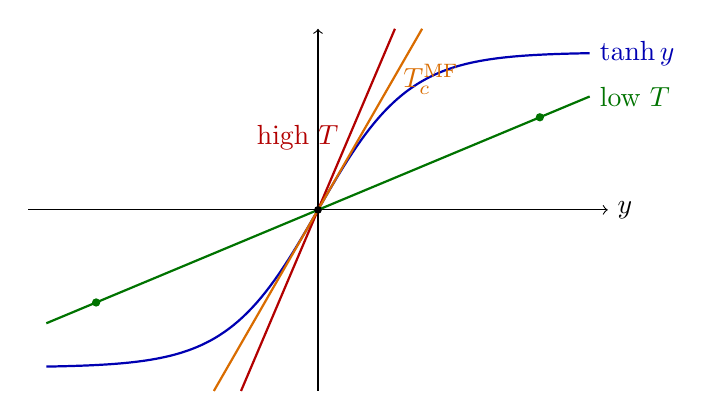
\begin{tikzpicture}[x=1.15cm,y=2.0cm]
\draw[->] (-3.2,0) -- (3.2,0) node[right] {$y$};
\draw[->] (0,-1.15) -- (0,1.15);
\draw[thick,blue!70!black,domain=-3:3,samples=120]
  plot (\x,{tanh(\x)}) node[right] {$\tanh y$};
\draw[thick,red!70!black] (-0.85,-1.15) -- (0.85,1.15)
  node[pos=0.70,left] {high \(T\)};
\draw[thick,orange!85!black] (-1.15,-1.15) -- (1.15,1.15)
  node[pos=0.86,right] {\(T_c^{\rm MF}\)};
\draw[thick,green!45!black] (-3,-0.72) -- (3,0.72)
  node[right] {low \(T\)};
\fill (0,0) circle (1.4pt);
\fill[green!45!black] (-2.45,-0.588) circle (1.5pt);
\fill[green!45!black] (2.45,0.588) circle (1.5pt);
\end{tikzpicture}TikZ, reconstruction normalisée de l’argument graphique d’autocohérence.\caption{}\end{figure}

La branche non nulle apparaît de manière continue. Près de la transition,
\begin{equation}
\tanh(Km)=Km-\frac{(Km)^3}{3}+O(m^5).
\end{equation}
Pour \(K>1\), les petites solutions non nulles vérifient
\begin{equation}
m^2\simeq \frac{3(K-1)}{K^3}.
\end{equation}
Le champ moyen prédit ainsi l’apparition caractéristique en racine carrée \(m\propto(T_c-T)^{1/2}\).

On peut aussi formuler la stabilité sans s’appuyer sur la représentation graphique. À une constante indépendante de \(m\) près, l’énergie libre de champ moyen par spin est
\begin{equation}
f_{\rm MF}(m)
=dJm^2-\frac{1}{\beta}
\log\!\left[2\cosh(2\beta dJm)\right].
\label{eq:mf-free-energy}
\end{equation}
Sa condition de stationnarité est
\begin{equation}
\frac{\partial f_{\rm MF}}{\partial m}
=2dJ\left[m-\tanh(2\beta dJm)\right]=0.
\end{equation}
Au-dessus de \(T_c^{\rm MF}\), \(m=0\) est le minimum. Au-dessous, l’origine est un maximum local et les deux solutions non nulles sont des minima dégénérés. La géométrie des intersections et la thermodynamique de l’énergie libre racontent la même chose.

\begin{classroomqa}\audiencequestion{La solution \(m=0\) demeure une intersection en dessous de \(T_c^{\rm MF}\). Pourquoi la branche non nulle serait-elle physique ?}\lecturerresponse{En remontant le système depuis la température nulle, on se trouve déjà sur une branche aimantée. Plus formellement, l’énergie libre de champ moyen présente des minima en \(\pm m_0\) sous la transition, tandis que \(m=0\) devient un maximum. Un champ extérieur infinitésimal sélectionne alors l’un des minima et lève l’ambiguïté apparente. \lecturetimestamp{01:11:34--01:12:18}}\end{classroomqa}

\section{Pourquoi le champ moyen échoue en une dimension}

Remplacer \(d=1\) dans l’équation~\eqref{eq:mean-field-tc} prédirait une transition à \(T=2J\), en contradiction avec la solution exacte unidimensionnelle. Aucun terme algébrique ne diverge. L’approximation échoue parce que deux voisins ne constituent pas un grand bain statistique et que les parois de domaine en une dimension ont une entropie exceptionnelle.

Partons de l’état où tous les spins sont orientés vers le haut. Une liaison rompue voit son énergie passer de \(-J\) à \(+J\) ; chaque liaison rompue coûte donc
\begin{equation}
\Delta E_{\rm bond}=2J.
\end{equation}
Sur un réseau carré, un spin retourné rompt quatre liaisons et coûte \(8J\). Deux spins retournés adjacents délimitent six liaisons rompues et coûtent \(12J\), tandis que deux spins retournés très éloignés en rompent huit et coûtent \(16J\).

\begin{figure}[ht]\centering
\includegraphics[width=0.82\textwidth]{lecture_09_figure_09.png}\caption{Deux spins retournés adjacents sur un réseau carré ; leur liaison commune est satisfaite, ce qui laisse un contour de six liaisons.}\lectureframe{01:17:30}\end{figure}

En deux dimensions, une goutte renversée compacte paie donc une énergie proportionnelle à la longueur de son contour :
\begin{equation}
\Delta E_{\rm 2d}=2J\,|\partial D|.
\end{equation}
La croissance de la goutte allonge généralement son contour.

La situation est différente en une dimension. Un bloc renversé contigu, quelle que soit sa longueur, ne comporte que deux parois de domaine :
\begin{equation}
\Delta E_{\rm 1d}=2(2J)=4J.
\label{eq:one-d-domain-cost}
\end{equation}

\begin{figure}[ht]\centering
\includegraphics[width=0.82\textwidth]{lecture_09_figure_10.png}\caption{Un long bloc renversé en une dimension, délimité par seulement deux parois de domaine.}\lectureframe{01:19:10}\end{figure}

Il existe de l’ordre de \(N^2\) façons de choisir les deux parois dans une chaîne de \(N\) sites. Leur énergie ne dépend pas de la distance qui les sépare. À toute température positive, l’entropie favorise donc des domaines renversés arbitrairement grands. En deux dimensions, à suffisamment basse température, l’énergie de contour peut l’emporter sur l’entropie des contours. Cette compétition entre énergie et entropie est une propriété géométrique que le champ moyen ne peut pas voir lorsqu’il traite \(d=1\) et \(d=2\) comme deux valeurs numériques d’un même coefficient.

\begin{classroomqa}\audiencequestion{Le coût constant associé aux deux parois exige-t-il que les spins retournés soient adjacents ?}\lecturerresponse{Oui. Cette affirmation porte sur un seul bloc renversé contigu. Si les spins retournés forment plusieurs blocs séparés, chaque bloc ajoute deux parois de domaine. Le point essentiel est qu’un seul bloc peut être arbitrairement long tout en ne comportant que deux parois. \lecturetimestamp{01:18:32--01:18:40}}\end{classroomqa}

\begin{classroomqa}\audiencequestion{L’équation de champ moyen elle-même ne semble faire aucune distinction qualitative entre \(d=1\) et \(d=2\). Est-ce là le problème ?}\lecturerresponse{Exactement. Le champ moyen prédit une transition pour tout \(d\) positif ; en une dimension, il est donc qualitativement erroné. Sa dérivation supposait de nombreux voisins dont les fluctuations sont faibles et négligeait la géométrie des parois de domaine. Pour le cas unidimensionnel, c’est la solution exacte en variables de liaison qui tranche, et non la substitution de champ moyen \(d=1\). \lecturetimestamp{01:19:44--01:20:28}}\end{classroomqa}

\section{Un champ extérieur sélectionne la phase}

Ajoutons un champ uniforme \(h\), en convenant que \(h>0\) favorise \(\sigma=+1\) :
\begin{equation}
H=-J\sum_{\langle ij\rangle}\sigma_i\sigma_j
-h\sum_i\sigma_i.
\label{eq:ising-with-field}
\end{equation}
L’énergie de champ moyen d’un spin choisi est
\begin{equation}
E_i^{\rm MF}=-(2dJm+h)\sigma_i,
\end{equation}
et l’équation d’autocohérence devient
\begin{equation}
\boxed{m=\tanh\!\left[\beta(2dJm+h)\right]}.
\label{eq:self-consistency-field}
\end{equation}
Avec \(K=2\beta dJ\) et \(y=Km\),
\begin{equation}
\frac{y}{K}=\tanh(y+\beta h).
\label{eq:shifted-graph}
\end{equation}

\begin{figure}[ht]\centering
\includegraphics[width=0.82\textwidth]{lecture_09_figure_11.png}\caption{Ajout du terme de champ extérieur à l’équation d’autocohérence et construction graphique décalée correspondante.}\lectureframe{01:26:20}\end{figure}

\begin{classroomqa}\audiencequestion{Pourquoi le champ est-il ajouté uniquement à l’intérieur de la tangente hyperbolique ? Ne devrait-il pas aussi modifier le membre de gauche ?}\lecturerresponse{Le membre de gauche est l’aimantation supposée \(m\), ou, de manière équivalente, \(y/K\). Le membre de droite est l’aimantation calculée pour un spin soumis au champ effectif total \(2dJm+h\). L’autocohérence impose l’égalité de ces deux quantités. En gardant \(y=Km\) comme définition, le nouveau terme ne figure que dans l’argument \(\tanh(y+\beta h)\). \lecturetimestamp{01:23:46--01:26:18}}\end{classroomqa}

\begin{classroomqa}\audiencequestion{Peut-on décrire le même changement graphique en déplaçant les droites plutôt qu’en décalant la courbe \(\tanh\) ?}\lecturerresponse{Oui. On peut garder \(\tanh y\) fixe et réécrire l’équation de sorte que la droite ait une ordonnée à l’origine non nulle. Les intersections sont identiques. Les deux descriptions diffèrent seulement par le choix du membre de l’équation représenté par la courbe fixe. \lecturetimestamp{01:35:07--01:36:26}}\end{classroomqa}

Pour \(h\neq0\), l’origine n’est plus une solution. En dessous de \(T_c^{\rm MF}\), un champ positif arbitrairement faible sélectionne la branche positive ; un champ négatif sélectionne la branche négative.

\begin{figure}[ht]\centering
\includegraphics[width=0.82\textwidth]{lecture_09_figure_12.png}\caption{Un faible champ supprime l’intersection symétrique et sélectionne l’une des branches aimantées.}\lectureframe{01:36:22}\end{figure}

Il faut préciser l’ordre des limites. Un système fini à \(h=0\) possède une symétrie par retournement des spins ; dans l’ensemble d’équilibre complet, il vérifie donc \(\expect{m}=0\). L’aimantation spontanée est définie par
\begin{equation}
m_{\rm sp}
=\lim_{h\to0^+}\lim_{N\to\infty}\expect{m}_{N,h},
\end{equation}
en prenant d’abord la limite thermodynamique. Inverser le signe du champ infinitésimal donne \(-m_{\rm sp}\). La différence d’énergie due au champ total est proportionnelle à \(Nh\) ; même un champ infime devient donc décisif pour un échantillon macroscopique.

L’énergie libre correspondante rend visible l’inclinaison :
\begin{equation}
f_{\rm MF}(m;h)
=dJm^2-\frac{1}{\beta}
\log\!\left[2\cosh\!\left(\beta(2dJm+h)\right)\right].
\end{equation}
À \(h=0\), les deux puits ont la même profondeur. Un champ positif \(h\) abaisse le puits associé à \(m\) positif et relève celui associé à \(m\) négatif. La perturbation par spin peut être infime, alors que la préférence totale, multipliée par \(N\), est macroscopique.

\begin{classroomqa}
\audiencequestion{Si le champ extérieur reste présent, l’aimantation est-elle vraiment spontanée ?}
\lecturerresponse{Le champ sert uniquement à sélectionner une branche. À \(T<T_c\) fixé, on porte le système à la limite thermodynamique, puis on prend la limite \(h\to0^+\). L’aimantation reste finie alors même que le champ de sélection s’annule. Inverser le signe de la limite sélectionne la phase opposée. \lecturetimestamp{01:33:15--01:34:18}}
\end{classroomqa}

\begin{classroomqa}
\audiencequestion{La solution de moyenne nulle est-elle réellement impossible sous la transition, ou est-elle seulement instable ?}
\lecturerresponse{À champ exactement nul, un ensemble statistique symétrique dans un volume fini, où les deux orientations ont le même poids, est possible et présente une moyenne nulle. Ce qui échoue, c’est sa stabilité en tant que phase macroscopique unique. Un champ, même arbitrairement faible, modifie le bilan énergétique extensif et sélectionne une orientation ; après la limite thermodynamique, l’aimantation sélectionnée subsiste lorsque le champ est supprimé. \lecturetimestamp{01:34:25--01:35:06}}
\end{classroomqa}

\begin{classroomqa}
\audiencequestion{Que devient la solution favorisée par le champ à température infinie ?}
\lecturerresponse{Pour tout \(h\) fini fixé, \(K=2\beta dJ\) et \(\beta h\) tendent tous deux vers zéro lorsque \(T\to\infty\). L’équation~\eqref{eq:self-consistency-field} donne alors \(m\to0\). Le faible champ sélectionne une branche de basse température, mais il ne peut maintenir l’ordre face à l’agitation thermique infinie. \lecturetimestamp{01:27:39--01:29:51}}
\end{classroomqa}

\begin{classroomqa}
\audiencequestion{Lorsque la température et le décalage du graphe varient simultanément, comment savoir où se déplace le point d’intersection ?}
\lecturerresponse{L’équation implicite est plus fiable que le schéma qui se déplace. À basse température et pour \(h\) positif, sa solution stable tend vers \(m=+1\). À haute température, le développement de la tangente donne
\[
m\simeq \beta(2dJm+h)
\quad\Longrightarrow\quad
m\simeq \frac{\beta h}{1-2\beta dJ},
\]
ce qui tend vers zéro lorsque \(\beta\to0\). La branche stable relie donc la limite alignée de basse température à la limite faiblement polarisée de haute température, sans rester à l’origine instable sous la transition. \lecturetimestamp{01:29:53--01:33:04}}
\end{classroomqa}

\section{L’inversion du champ magnétique est un problème différent}

\begin{classroomqa}
\audiencequestion{Qu’est-ce qui provoque l’inversion du champ magnétique terrestre ?}
\lecturerresponse{Cette question dépasse le cadre du modèle d’Ising à l’équilibre. Le champ magnétique principal de la Terre est produit par la géodynamo : la convection et la rotation du fluide électriquement conducteur du noyau externe entretiennent des courants électriques et un champ magnétique. Les inversions sont des réorganisations irrégulières de cette dynamo non linéaire, et non un simple retournement des domaines ferromagnétiques dans du fer solide. Leur chronologie détaillée ne se décrit pas au moyen d’un unique paramètre d’ordre à l’équilibre ; la réponse honnête est donc que le calcul d’Ising n’explique pas le déclenchement. Le seul lien utile est général : un système possédant deux orientations opposées à grande échelle peut connaître une instabilité entre celles-ci.\footnote{Voir la \href{https://science.nasa.gov/science-research/earth-science/earths-magnetosphere-protecting-our-planet-from-harmful-space-energy/}{présentation de la géodynamo par la NASA} et l’\href{https://www.usgs.gov/programs/geomagnetism/introduction-geomagnetism}{introduction au géomagnétisme de l’USGS}.} \lecturetimestamp{01:38:39--01:40:32}}
\end{classroomqa}

La chaîne exacte et le réseau traité en champ moyen donnent maintenant deux réponses très différentes. En une dimension,
\begin{equation}
\expect{\sigma_i\sigma_{i+r}}
=\left[\tanh(\beta J)\right]^r
\longrightarrow0
\qquad (T>0),
\end{equation}
car des parois de domaine d’énergie finie peuvent séparer des intervalles inversés de longueur arbitraire. Avec un grand nombre de voisins, le champ autocohérent admet au contraire des solutions non nulles stables au-dessous de
\begin{equation}
T_c^{\rm MF}=2dJ.
\end{equation}
Le contraste n’est pas simplement algébrique. Il tient à la compétition entre la géométrie, l’énergie, l’entropie et la redondance : une erreur peut-elle se propager librement, ou le réseau environnant peut-il la corriger ?
